%auto-ignore
%      this ensures the arxiv doesn't try to start TeXing here.
%!TEX root = super_lattice_models_draft.tex
%      prev line helps TeXShop do the right thing



%%%%%%%%%%%%%%%%%%%%%%%
\section{Super pivotal state sums and tensor networks} \label{state_sums}
%%%%%%%%%%%%%%%%%%%%%%%

\dave{Note to self: look at \cite{beliakova1998} and check for relations.}

In this section we write down a Turaev-Viro-Barrett-Westbury (TVBW) state sum \cite{Turaev1992,Barrett1996}
for the super pivotal fusion categories, 
and a tensor network for the ground state wave function of the Hamiltonian constructed in Section \ref{Super_pivotal_Hamiltonian}.
%\eqref{ham}.
%Very closely related 
Related 
%\kw{very closely related, or just related?
%I could not tell after a quick look at the paper.}
work was presented in~\cite{bhardwaj2016}, 
see also \cite{Bultinck2017, upcoming-paper?}.
\kw{fix citation}
We first review the TVBW construction for bosonic spherical fusion categories. 
We then show how to write the state-sum as a tensor contraction on a tensor 
network.
Next we detail the modifications needed for the fermionic versions of the state sum and tensor network.
%which allows us to extend the state-sum to the super-pivotal case with only minor modifications.
Lastly we use the state sum to write down an explicit wave function for the ground ground state of \eqref{ham}.

\medskip

Before we begin, we need to establish some terminology regarding cell and handle decompositions. 
Recall that a handle decomposition for a 
3-manifold $M$ is built from a series of $k$-handles, with $k=0,1,2,3$, each of which is identified with $D^k\times D^{3-k}$. 
Handle decompositions can be obtained from cell decompositions by thickening each $k$-cell into a $k$-handle.
Conversely, each handle decomposition determines a cell decomposition by taking the cores of the handles.
(See Section \ref{standardized_handles} for more details.)
%Each $k$-handle is obtained from a $k$-cell by ``fattening'' the $k$-cell in the manner described 
%in Section \ref{standardized_handles}.
We will often refer to a $k$-cell and its associated $k$-handle with the same letter, since
it will be convenient for us to be able to describe things in terms of both handle decompositions 
and their corresponding cell decompositions. 
We call $S^{k-1} \times D^{3-k}$ the attaching region (or attaching boundary) of the $k$-handle,
and $D^k\times S^{3-k-1}$ the non-attaching boundary.
%The attaching region of a $k$-handle is $S^{k-1} \times D^{3-k}$,
The attaching map of a $k$-handle is a homeomorphism from the attaching region to 
a submanifold of the boundary of the union of the lower-dimensional handles.
The topology of $M$ is encoded by the various attaching maps.
\dave{Maybe draw a figure showing 0-, 1-, 2- and 3-cells and the corresponding 0- 1-, 2- and 3-handles.
\ref{cell_and_handle_decomp}}
\begin{figure}
\begin{align}
\text{a figure} 
\end{align}
\caption{
\label{cell_and_handle_decomp}
Here we show part of a cell decomposition and its associated handle decomposition. 
An example of each k-cell, and k-handle is shown...
Note orientations etc.
}
\end{figure}


\kw{to do: restore description on relation of cell decomps to handle decomps; also establish conventions for manifolds
with boundary}


%%%%%%%%%%%%%%%%%%%%
\subsection{Bosonic TVBW state sum}
%%%%%%%%%%%%%%%%%%%%

\subsubsection{Definition of the state sum}


Our first task is to describe the TVBW (bosonic) state sum.
The original references are \cite{Turaev1992,Barrett1996}.
We will use the form for a general cell/handle decomposition, as described in \cite{Walker2006}.

Let $M$ be a closed oriented 3-manifold equipped with a handle decomposition $\mch$.
Choose auxiliary orientations of the 1- and 2-cells of the cell decomposition corresponding to $\mch$.
Let $\mch_i$ denote the set of $i$-handles ($i = 0,1,2,3$).
The state sum has the form
\be \label{bos_tv_sum}
	Z(M) = \sum_{\beta\in\mcl(\mch)}
		\prod_{c\in\mch_3} \mcd^{-2}
		\prod_{f\in\mch_2} d(f, \beta)
		\prod_{e\in\mch_1} \widetilde\Theta(e, \beta)^{-1}
		\prod_{v\in\mch_0} \text{Link}(v, \beta) .
\ee
The next few paragraphs define the notation used in \eqref{bos_tv_sum}.

\begin{figure}
\begin{center} 
\begin{align}
\nonumber
\TwoHandleToGraph
\end{align}
\caption{\label{TwoHandleToGraph}
\dave{Just draw attaching graph on 2-handle (no 2-cell). 
Remove all 2-cells.}
\ethan{so, let's delete the left figure and keep the right one.}
A triangular 2-cell and its adjacent 0- and 1- and 2- handles. 
The oriented 2-cell determines part of the graphs on each 0-, 1- and 2-handle. 
In the figure, we show the part of the graphs on each 0- and 1-handle determined by the 2-cell.
The attachment regions on the 1- and 0-handles that do not intersect the shaded 2-cell have been omitted for clarity.}
\end{center} 
\end{figure} 

We use the 2-cell orientations to define an oriented graph (unlabeled string net) on the boundary of each 0-, 1- and 2-handle,
as shown in Figure \ref{TwoHandleToGraph}.
String-net graphs are assigned to the $k$-handles as follows:
\kw{KW to-do: maybe draw another fig for this}
\begin{itemize}
\item On 2-handles, the graph is a single loop along the core of the attaching annulus of a 2-handle.
The orientation of the loop is determined by the orientation of the 2-cell. 
%For a 2-cell 
%$f$, this is shown in the top left of Figure \ref{NotationStateSum}. \ethan{may wan to remove the $c_{fe}$ stuff from the figure}
\item On 1-handles, the graph is a generalized $\Theta$ graph, which we will call a $\widetilde\Theta$ graph.
The graph has one edge for each 2-handle adjacent to the 1-handle.
The middle part of each edge of the graph corresponds to where the cores of the 2-handles meet the boundary of the 1-handle.
The two vertices of the graph are on the two attaching disks of the 1-handle.
The edges are oriented opposite to the orientations used in the 2-handle loops above.
\item On each 0-handle, the graph is determined by the pattern of 2- and 1-handles adjacent to the 0-handle.
The graph has one edge for each adjacent 2-handle and one vertex for each adjacent 1-handle.
The orientations of the edges are opposite to the orientations of the 2-handle loops.
We denote this graph $\text{Link}(v)$.
\end{itemize}

\begin{figure}
\centering
\begin{align}
\nonumber
\CellDecompNearOneHandle \quad \quad \quad \quad \quad \OneHandlePrime 
\end{align}
\caption{\label{OneHandlePrime}
On the left, we have an illustration of four 2-cells meeting a 1-cell.
For clarity we have put a small gap between the 1-cell and the four 2-cells.
On the right we have the corresponding 1-handle and a particular labeling. 
We have denoted the corresponding attaching disks by `i' for initial, and `t' for terminal. 
}
\end{figure}

Recall that we have an orientation of each 1-cell.
This allows us to distinguish an ``initial" and ``terminal" attaching disk for each 1-handle; see Figure \ref{OneHandlePrime}.
On the initial disk we see a graph with a single vertex in the interior of the disk and $k$ edges connecting the central vertex
to the boundary of the disk (where $k$ is the number of 2-handles which cross the 1-handle).
For each labeling $\ell$ of these edges by simple objects in $\sob(\mcc)$, we have an associated vector space $V(\ell)$.
For example, in the case of Figure \ref{OneHandlePrime} the vector space is isomorphic to $V^{ab^*c^*d}$.
Let $B(\ell)$ be some chosen basis of this vector space.
For each 1-handle $e$ define $B(e)$ to be the union over all labelings $\ell$ of $B(\ell)$,
and also define $V(e)$ to be the direct sum of all the vector spaces $V(\ell)$.

We define the set of all labelings $\mcl(\mch)$ to be the product over all 1-handles $e$ of the basis sets $B(e)$.
In other words, we choose (independently, without any compatibility constraints) a labeling by simple objects of the edges of each initial
disk graph, then choose a basis vector for each associated vector space.

We also associate a vector space $V^*(\ell)$ to the terminal disk of each labeled 1-handle.
%\dave{Should we use a different star here? 
%Since it is somewhat different than the two stars we defined in the definition section.
%Or maybe we should just use $V^i(e)$ and $V^t(e)$ for initial and terminal vector spaces. 
%Then use $(V^i(e))^*$ and $(V^t(e))^*$ for their respective duals as defined by the `standard' reflection pairing (input vector spaces to $\text{Link}(v)$.)
%}
%\dave{I retract this comment.}
In the example, this is isomorphic to $V^{d^*cba^*}$.
%In the example, this is isomorphic to $(V^{a^*bc^*})^*$.
%We also define $V^*(e)$ to be the direct sum (over all labelings $b$) of $V^*(\ell)$.
There is a nondegenerate bilinear pairing between $V(\ell)$ and $V^*(\ell)$, 
given by evaluating the labeled string net on the boundary of the 1-handle (which is a 2-sphere).
%(This is closely related to the pairing \eqref{reflection_pairing_defn}.)
%found by applying the standard bilinear pairing \eqref{reflection_pairing_defn} after a rigid translation through the 1-handle.
%\eqref{reflection_pairing_defn} and 
%graphically looks like a banana. % :--)
%\ethan{we should probably change $\mcb$ to $\Theta$ or the other way around to make notation consistent}
%\dave{Or should we change $\mcb$ to $\widetilde{\Theta}$ and save $\Theta$ for trivalent junctions?}
%\dave{Need to consider whether we put the pivots on the 1-handles or the 0-handles.}
%\ethan{whether we want a back reference to $\mcb$ is tbd}
We will choose a basis of $V^*(\ell)$ such that the pairing matrix is diagonal.
(It is sometimes convenient to not insist that the diagonal entries be $\delta_{ij}$.)
%As with $\mcb$, it is sometimes convenient to not insist that the diagonal entries be $\delta_{ij}$.
We also define $V^*(e)$ to be the direct sum (over all labelings $\ell$) of $V^*(\ell)$.

We are now ready to define the weights appearing in the state-sum $Z(M)$. 
Let $\beta\in\mcl(\mch)$ and let $f$ be a 2-handle.
The labeling $\beta$ associates a simple object to each intersection of $f$ with a 1-handle.
If these simple objects are not all the same, we define $d(f, \beta) = 0$.
If they are all equal to the same simple object $a\in\sob(\mcc)$, we define the weight $d(f, \beta)$
appearing in \eqref{bos_tv_sum} by $d(f,\beta) = d_a$.

Let $e$ be a 1-handle.
The labeling $\beta$ associates a basis vector $\mu$ to the initial disk of $e$.
Define $\widetilde\Theta(e, \beta)$ to be the value of the bilinear pairing evaluated on $\mu^*$ and $\mu$.
%\dave{I'm guessing with this convention we have cut the 1-handle between the two 0-handles. 
%Otherwise if we cut at the ends near the 0-handles we need $\widetilde{\Theta}  \ra \frac{\widetilde{\Theta}\widetilde{\Theta}  }{ \widetilde{\Theta} } $ in $\widetilde\theta$ in $Z(M)$.
%Two standard ones coming from the attaching disks of the 1-handle, and one non-standard one that depends on the 1-handle itself (e.g., could have a pivot).
%Is that correct? Should we mention this?
%}
Diagrammatically, $\widetilde\Theta(e, \beta)$ is found by connecting the open strings in $V(\ell)$ to their dual counterparts in $V^*(\ell)$ and evaluating 
the resulting diagram.
Continuing with our example in Figure \ref{OneHandlePrime}, 
%%KW 2-handles don't get directly labeled
%if $e$ has four adjacent 2-handles labeled by $a,b,c,d$ with the orientations of Figure \ref{OneHandlePrime} so that $\mu \in V^{ab^*c^*d}$, then 
we have 
\be \widetilde \Theta (e, \beta) =  \Bananafourmu.
\ee
%\ethan{need to change $\eta_i$ in the fig to $\mu^*$ and $\mu$}
%\dave{done}


Let $v$ be a 0-handle.
The labeling $\beta$ determines a labeling of the graph $\text{Link}(v)$ as follows.
Near each vertex of $\text{Link}(v)$ we place the basis element $\mu^* \in V^*(e)$ (or $\mu \in V(e)$) assigned by $\beta$ to the 
corresponding 1-handle if $v$ is attached to the initial (terminal) end of the 1-handle.
%\footnote{The dual spaces here are determined by the bilinear pairing of \eqref{reflection_pairing_defn}.}
%\dave{I think it should be $\mu^* \in V(e)^*$ and $\mu \in (V^*(e))^*$.}
%\ethan{to make it consistent with our earlier writing of the section, I think yes. I interchanged them.}
If these vertex labels are incompatible along edges of $\text{Link}(v)$, we define $\text{Link}(v, \beta) = 0$.
If they are all compatible then we define $\text{Link}(v, \beta)$ to be the evaluation of the resulting labeled graph (string net).
%\ethan{The evaluation is zero if they aren't compatible, so we can just say it's the evaluation and leave it at that.}
%\kw{I would say the evaluation is not defined if the labels do not match.}
For cell decompositions dual to a triangulation, 
the labeled graph is a tetrahedral string net on a sphere.
This is illustrated in Figure \ref{to be filled in}, which shows an example 0-handle on which 
four 1-handles terminate. The attaching regions for the 1-handles are marked in green, and those 
for the two-handles are marked in purple. $\beta$ assigns string-net labels to the purple strips and 
basis elements $\mu$ to the green regions, with ${\rm Link}(v,\beta)$ being computed by evaluating the resulting graph on the sphere. 

\begin{align}
\TetSphereColored
\end{align}
\dave{need to add orientations}
\ethan{I would say make into figure rather than eqn.}
%these string nets take the form 
%of tetrahedral symbols. 
%\dave{I think tetrahedral symbol is a bit of a loaded term, so I re-worded.}

This completes the definition of the state sum.

\medskip

It follows from Section 8.2 of \cite{Walker2006} that the state sum computes $Z(M)$, independently of the choice of handle decomposition
and choice of orientations of 1- and 2-cells.

\medskip

If $M$ has non-empty boundary,
we choose the handle decomposition to have the form shown in Figure xxx near the boundary.
In terms of cell decompositions, we choose a cell decomposition such that $\bd M$ lies in the 2-skeleton, rather
than a cell decomposition such $\bd M$ is transverse to the cells.

The 0- and 1-cells on $\bd M$ will do double duty as the underlying graph of a string net on $\bd M$.
Choose an orientation of each 1-cell on $\bd M$.
(This is analogous to choosing an orientation of the boundary of a 2-cell in the interior of $M$.)
Choose a labeling of these oriented edges by simple objects in $\sob(\mcc)$.
For each vertex (0-cell) on $\bd M$, choose an element of the appropriate disk vector space
(e.g.\ $V^{ab}_c$ in Figure xxxx).

We now have a labeled string net $g$ on $\bd M$.
The state sum will evaluate the path integral $Z(M)(g)$ 
(i.e.\ the path integral of $M$ with boundary condition given by $g$).
The labelings and weights are defined as before, except that some of the labels are already determined by the string net $g$ on the boundary.

%%KW accidentally rewrote this above; not sure which version is better.
%We also choose a string net on $\bd M$ compatible with the handle decomposition (a labeled edge
%for each 1-handle along $\bd M$, and a labeled vertex for each 0-handle along $\bd M$).
%We modify the label set $\mcl(\mch)$ to be fixed for strands on $\bd M$ and varying for interior labels.
%The modified state sum assigns a number to each fixed boundary string net.
%This can be interpreted as a linear function $A(\bd M)\to\cc$ (i.e., a wavefunction).
%%which gives us a wavefunction, i.e. linear function $A(\bd M)\to\cc$.

%\dave{Maybe think about reference to wavefunction.}


%%%%%%%%%%%%%%%%%%%%%%%%%
\subsubsection{The state sum as a tensor network}
%%%%%%%%%%%%%%%%%%%%%%%%%

Our goal in this subsection is to reinterpret \eqref{bos_tv_sum} as a tensor network.
We will first discuss that case when $M$ is closed, then consider the case when $\bd M$ is non-empty.
%\ethan{replaced ``regularization'' with ``standardization'' since regularization has a different physics meaning}
%\dave{Definitely a good idea.}

\medskip

If we (temporarily) ignore the factors of $d(f, \beta)$ and $\mcd^{-2}$ in \eqref{bos_tv_sum}, 
it is easily seen to compute the contraction of a tensor network.
%it is easy to see that it computes the tensor contraction of a tensor network.
The underlying graph of the tensor network is the union of 0- and 1-cells of the cell decomposition.
The vector space associated to each edge $e$ is $V(e)$ as defined above.
The matrix elements of the tensor associated to a 0-cell $v$ are the numbers $\text{Link}(v, \beta)$ defined above.
The factors of $\widetilde\Theta(e, \beta)^{-1}$ arise from the pairing of dual tensor indices.
%\kw{Say more about this?}
%\kw{remark about dual spaces here??}
%\dave{What did you have in mind?}

To incorporate the factors of $d(f, \beta)$ and $\mcd^{-2}$, we make some ad hoc choices.
We consider ``dressed" 
%\kw{Is this the usual meaning of ``dressed"?  If so, great.}
%\dave{If you are happy with thinking of $d(f, \beta)$ and $\mcd^{-2}$ as being clothes for $\text{Link}(v,\beta)$ then, yes. 
%But more seriously. I don't think it has a super established meaning, and don't think it would raise eyebrows. 
%I think in a lot of the physics literature it appears as ``dressing'' domain walls.
%It's sometimes used to avoid writing down an explicit Hamiltonian and only talking about the physics of a hypothetical Hamiltonian. 
%}
0-handle weights that tack on the factors of $d(f,\beta)$ and $\mcd^{-2}$.
For each 2-handle $f$ we choose an adjacent 0-handle $v_f$.
For a 0-handle $v$ we modify the associated weight ${\text{Link}}(v,\beta)$ by multiplying factors of $d(f,\beta)$ for each 2-handle $f$ such that $v = v_f$.
Similarly, for each 3-handle we choose an adjacent 0-handle and multiply the associated weight by $\mcd^{-2}$.
Denoting the modified 0-handle weights by $\widetilde{\rm Link}(v,\beta)$, 
we define the 0-handle tensors $T_v$ as follows.
Let $e_1, \ldots, e_k$ be the 1-handles adjacent to the 0-handle $v$.
Let 
\begin{align}
\label{0_handleVectorspaces}
V_i = \begin{cases}
V(e_i) & \text{if $v$ is adjacent to the terminal end of $e_i$}\\
V^*(e_i) & \text{ if $v$ is adjacent to the initial end of $e_i$}.\\
\end{cases}
\end{align}
%Let $V_i$ be either $V(e_i)$ (if $v$ is adjacent to the terminal end of $e_i$)
%or $V^*(e_i)$ (if $v$ is adjacent to the initial end of $e_i$).
We define
\be
	T_v \in V^*_1\tp\cdots\tp V^*_k
\ee
by
\be
\label{vertex_tensor}
	T_v(w_1\tp\cdots\tp w_k) = \widetilde{\text{Link}}(v, w_1\tp\cdots\tp w_k),
\ee
where $w_i\in V_i$.
In other words, $T_v$ evaluates the link graph with labels determined by $w_1,\ldots,w_k$ and multiplied by the factors of $d(f,\beta)$ and $\mcd^{-2}$ as described above.
%\kw{... end ``as follows"}
%\dave{Is this necessary?}
%\ethan{It was intended to be my guess to what Kevin's dual spaces comment meant. Might have missed the mark though, and it might still be confusing.}
To obtain the partition function, we trace out the tensor product of all the 0-handle tensors constructed in this way.
Because the vector space associated to the region on a $0$-handle attached to the 
terminal end of a 1-handle $e$ is dual to the vector space associated to the corresponding region on the 
0-handle attached to the initial end of $e$, there are precisely as many dual vectors as vectors in the tensor product, and 
contracting each vector with its associated dual vector computes the complex number $Z(M)$. 
That is, we have 
%\ethan{I think we need something like this. If you guys don't like tTr then we can use an appropriately normalized $\Theta$ instead}
%\dave{I like ${\rm tTr}$ for now.
%We do need to define it though.}
%\kw{Maybe $\text{tc}$ for tensor contraction?}
%\dave{I think Gu-Levin-Wen used ${\rm tTr}$ (in a similar context), which is one reason to stick with it. 
%Although would have to check if it's been used much since.
%Sometimes people use $C( ....) $ for contraction, or even $\mcc(...)$. 
%Both of those would probably be a nuisance in this paper though. 
%$tc$ for tensor contract is nice, my only reservation is that there is probably a few other notations that have been established. 
%}
%\dave{It's kind of like $\text{eval}^{-1}$. 
%Is there a standard tensor category name for that?}
%\kw{If tTr is well established, then fine.  Otherwise maybe a simple tr would do.
%I think tr is often used in this generalized sense in math papers.}
%\dave{I talked to one friend, he didn't think there was any well established notation for this. }
\be Z(M) = \tr \left(\bigotimes_{v\in \mch_0} T_v\right),\ee
where the trace $\tr$ denotes the tensor contraction.
%%KW not sure why this remark is necessary; also ``normalized" doesn't seem like the right word.
%It is normalized so that a factor of $\widetilde{\Theta}^{-1}$ is introduced if the labels on each side of the 1-cell are dual to one another (with respect to the bilinear pairing) and is zero otherwise.\footnote{Alternatively we could use the standard pairing but then we would have to modify our vertex tensors by $T_v(w_1\tp\cdots\tp w_k) \ra T_v(w_1\tp\cdots\tp w_k) \widetilde{\Theta}(e_1,w_1)^{-1} \cdots \widetilde{\Theta}(e_k,w_k)^{-1}$  }
%\dave{May want to be more explicit.}
%\kw{This may have already been discussed above}
%\dave{I'll keep an eye out.}
It is easy to see that this tensor network gives the same state sum as \eqref{bos_tv_sum} and 
is independent of the way we assign factors of $d(f,\beta)$ and $\mcd^{-2}$ to the 
vertex tensors. 

\medskip

%In the case where $\partial M \neq \emptyset$, the Hilbert space associated 
%with the tensor product of the 0-cell tensors admits a decomposition $\mch^*_{bulk} \tp \mch_{bulk} \tp \mch(\bd M)$, where 
%the Hilbert spaces of the degrees of freedom on $\partial M$ lack dual tensor factors appearing in the tensor product. 
%The partition function is still performed by contracting, which contracts out the tensor factors in $\mch^*_{bulk} \tp \mch_{bulk}$ but leaves those in $\mch(\partial M)$ uncontracted, producing a wavefunction supported on $\mch(\partial M)$ (that is, a map $A(\partial M) \ra \cc$).
%\kw{This is basically correct, but let's work on the phrasing.}

%\dave{This version looks good to me.
%I'll come back to this}
In the case where $\partial M \neq \emptyset$, we define the 0-handle tensors $T_v$ as before,
but in this case some of the legs of the tensors are unpaired (not contracted).
Specifically, there is one unpaired leg for each 0-cell on $\bd M$.
If $W_1, \ldots, W_n$ are the vector spaces associated to the boundary 0-cells, we have
\be \label{trace_pM_nonempty}
	Z(M) = \tr \left( \bigotimes_{v\in \mch_0} T_v \right) \in W_1^*\tp\cdots\tp W_n^* .
\ee
Each string net on $\bd M$ (i.e. each labeling of 0- and 1-cells as described above)
determines an element of $W_1\tp\cdots\tp W_n$ (the vertex labels).
By evaluating \eqref{trace_pM_nonempty} on this element we obtain the value of the wave function for the string net.
\kw{rephrased the end of this paragraph}
\ethan{I like the new sentence} 
%The above tensor contraction provides a way to associate these string nets 
%with complex numbers, and
%produces the wave function on this space.


%%%%%%%%%%%%%%%%%
\subsubsection{Standardization procedures}
%%%%%%%%%%%%%%%%%

The above tensor network construction is irregular, in the sense that (potentially) every edge vector space is different 
and every 0-handle tensor is different.
There are several standardization procedures that reduce this irregularity. 

One standardization procedure is to start with a cell decomposition that is dual to a triangulation.
This ensures that there are exactly three 2-handles meeting each edge, and that the vertex graphs $\text{Link}(v,\beta)$ are all tetrahedral.
%However, this still leaves us with many different types of $k$-cell string nets.
However, this still leaves us with several diferent types of edge vector spaces and vertex tensors.
For example, depending on the choice of 1- and 2-cell orientations, there will be eight possible vector spaces associated to 1-handles,
corresponding to $V^{abc}$, $V^{ab^*c}$, $V^{a^*b^*c^*}$, etc.
(Note that if all Frobenius-Schur indicators are equal to 1, then we can ignore these differences.)
Similarly, there will be many different tetrahedral vertex tensors, depending on the orientations of the edges of the tetrahedral graph.

We can further standardize the tensor network by choosing a global ordering of the 3-cells of the handle decomposition.
%\dave{Lets add picture.}
%\ethan{personally I don't think we need figures for this paragraph, since we are never actually using this standardization convention, just mentioning it in passing}
%\dave{I agree.}
(This is equivalent to a global ordering of the vertices of the dual triangulation.)
We then choose 2-cell orientations so that the the orientation of a 2-cell together with a normal vector pointing toward the higher-ordered of the two
adjacent 3-cells agrees with the orientation of $M$.
%\dave{I'm confused, how can the 2-cells have an orientation that agrees with $M$? (the 2-handles can but then the sentence isn't making a lot of sense.)}
%\kw{2-cell orientation plue normal direction orientation; these two combine to give a 3d orientation}
%\dave{Thanks.}
We can now choose 1-cell orientations so that the graph on the initial disk of each 1-handle has a trivalent vertex with two
outgoing and one incoming edge.
With these orientation choices, we have, for every 1-handle $e$,
\be
	V(e) = \bigoplus_{a,b,c\in\sob(\mcc)} V^{abc^*} .
\ee
Furthermore, all of the tetrahedral graphs have the same pattern of edge orientations, so all of the 0-handle tensors
in the tensor network are of the same form. 

However, it is not always convenient to choose a global ordering.
For example, our main application is a tensor network associated to $Y\times I$.
If $Y$ is a torus, we might hope that the network has translational symmetry, but this is not compatible with the global ordering trick.
For this reason, in what follows we will work with a cell decomposition dual to a triangulation, but we will not employ the global ordering trick.

In what follows, we will find it useful to employ a standardization 
procedure in which all fusion spaces in the string nets assigned to the 0-handles 
assume the ``pitchfork'' form introduced 
in our treatment of the Hamiltonian. 
(These vertices are all trivalent since we are now 
assuming a cell decomposition dual to a triangulation.)
In this convention, the $T_v$ tensor weights are all computed by the evaluation of tetrahedral diagrams:
%\ethan{Actually, now I think the Tet notation isn't necessary.}
\begin{align} 
\label{Bosonic_tet}
	%T_v = \TetrahedronPrime \; \cdot \alpha \tp \beta \tp \gamma \tp \delta, 
	T_v(\alpha \tp \beta \tp \gamma \tp \delta) = {\rm Tet}(v,\alpha \tp \beta \tp \gamma \tp \delta) = \TetrahedronPrime , 
\end{align}
where we have defined the tensor weight by its evaluation of the picture on the right with 
$\alpha \in \bigoplus_{abc} V^{abc}$, $\beta \in \bigoplus_{a^* bc} V^{a^* bc}$, $\gamma \in \bigoplus_{a^* b c^*} V^{a^* b c^*}$, and $ \delta \in \bigoplus_{a^* b^* c^*} V^{a^* b^* c^*}$.
The pitchforkization procedure does not entirely fix the form of the $T_v$ tensors above, 
since the tetrahedral nets associated with each 0-handle will in general have different 
edge orientations.  
Since there are $2^6 = 64$ possible choices of edge orientations near a 0-handle, there will be 64 
different types of $T_v$ tensors, given by the appropriate diagram evaluation with $\alpha,\beta,\gamma,\delta$ chosen from the appropriate fusion spaces.%
\footnote{Not all these $64$ tetrahedra are independent however, as 
some of them can be transformed into one another by using the pivotal and spherical structure of the input category.}

In this procedure, we choose standardizations (pitchforkizations) at each 0-handle independently.
This means that the two ends of each 1-handle are standardized independently 
of each other, and the pairing induced from the $\widetilde\Theta$ graph on the 1-handle (Figure xxxx above \kw{fix ref})
will not necessarily agree with the standard pairing \eqref{reflection_pairing_defn}.
%This means that the form of a given trivalent vertex at the initial edge of a 1-handle $e$
%will not in general be the same as the form of the associated vertex on the terminal edge of the 1-handle:
Instead, the 1-handle pairing and the standard pairing will be 
related by a pivot operation $P_e=P^{l_e}$ for $l_e = 0,1,2$, where $P$ is the pivot defined in \eqref{Pitchfork_pivot}.
We define $P_e$ to rotate diagrams counterclockwise relative to the orientation of $e$. 
If $l_e \neq 0$, then the initial and terminal vertices of $e$ are twisted by $2\pi l_e / 3$ relative to 
one another, and this twisting data needs to be incorporated into the 1-handles. 
The 1-handles now look like
\begin{align} \label{horshoe_resln} 
\HorshoeIdentity, 
\end{align}
where the double arrows designate the orientation of $e$. 

%In summary, by standardizing the 0-handles, we have been forced to put extra data on each 1-handle, namely the pivots. 
%The 1-handle terms in the partition function (and corresponding tensor trace) also need to be modified.
%For a given labeling $\beta \in \mcl(\mch)$ we have two $\widetilde{\Theta}$ symbols associated with the initial and terminal disks of each 1-handle, and a matrix element of $P_e$.
%The matrix element of $P_e$ appears on the numerator, while the two $\widetilde{\Theta}$ symbols appear on the denominator.

In summary, by standardizing each 0-handle independently, we have managed to make each
0-handle tensor isomorphic to a standard (up to edge orientations) tetrahedral tensor.
The price we pay for this is that we have to keep track of the pivots which relate the two ends of each 1-handle.
In terms of the tensor network, this means that we either need to insert two-legged pivot/1-handle tensors between each pair
or adjacent 0-handle tensors, or we need to further ``dress" the 0-handle tensors by merging each such pivot tensor
into one of the two adjacent 0-handle tensors.
\kw{Figure for this?}
\dave{Were you thinking of a 2part figure. LHS has twisted 1-handle attaching two disks, and the other has an un-twisted 1-handle but a twist on one of the disks?}
\kw{Say that we will go with the first option?}
\dave{Probably. 
We already have (effectively) put tensors on the 1-handles corresponding to the $\widetilde{\Theta}$ symbols.}

\medskip

These standardizations also serve to make the original state sum \eqref{bos_tv_sum} more uniform.
We can now write
\be \label{bos_tv_sum_std}
	Z(M) = \sum_{\beta\in\mcl(\mch)}
		\prod_{c\in\mch_3} \mcd^{-2}
		\prod_{f\in\mch_2} d(f, \beta)
		\prod_{e\in\mch_1} \Theta(P_e, \beta)^{-1}
		\prod_{v\in\mch_0} \text{Tet}(v, \beta) .
\ee
Here $\Theta(P_e, \beta)$ is a standard pairing as in \eqref{reflection_pairing_defn}, but modified by the pivot isomorphism $P_e$.
The weight $\text{Tet}(v, \beta)$ is a standard tetrahedral symbol (though there are still variants which depend on
the orientations of the edges of the tetrahedron).
The point is that we have now written the state sum for an arbitrary 3-manifold in terms of a finite number
of standard weights.



%%%%%%%%%%%%%%%%%%%%%
\subsection{The fermionic state sum}
%%%%%%%%%%%%%%%%%%%%%

\subsubsection{Definition of the fermionic state sum}

We now extend the bosonic state sum to the fermionic case. 
We start with two pieces of data: a super pivotal fusion category $\spc$, and a spin % spin implies oriented
3-manifold $M$ possessing a cell decomposition with orientations of 1- and 2-cells.
%The fermionic version of the state sum can be computed using similar techniques as in the bosonic case,
%and takes the form
The fermionic version of the state sum is similar to the bosonic version:
\begin{align}
\label{fermionic_tv_sum}
	Z(M) = \sum_{\beta\in\mcl(\mch)}(-1)^{\kappa_\beta}
		\prod_{c\in\mch_3} \mcd^{-2}
		\prod_{f\in\mch_2} \frac{d(f, \beta)}{n(f,\beta)}
		%\prod_{e\in\mch_1} \frac{ (-1)^{F(e,\sigma, \beta)}}{ \widetilde \Theta(e, \beta)}
		\prod_{e\in\mch_1}  \widetilde \Theta(e, \beta)^{-1}
		\prod_{v\in\mch_0} \text{Link}(v, \beta) .
\end{align}
There are several important -- often subtle --  differences built into the fermionic state sum which don't appear in the bosonic one, namely:
\begin{itemize} 
\item %The 0- and 1-handle weights are linear functionals on super vector spaces and as such have a sign ordering associated to each tensor.
The the string nets corresponding to the 0- and 1-handle weights require a sign-ordering of their string net vertices. 
This in turn requires that the partition function is weighted by a Koszul sign $(-1)^{\kappa_\beta}$
which measures the difference between the global sign ordering coming from the 1-handles and the global sign ordering coming from the 0-handles.
%\dave{That's a nice way to phrase it.}
\item The weights assigned to the 2-handles need to be properly normalized, 
resulting in a factor of $n(f,\beta) = \dim \End(a)$ if $a$ is the simple object labeling the core of the attaching annulus for the 2-handle $f$ by $\beta$.
%\item The spin structure on $M$ is determined by the spin structure on the 0- and 1-handles, 
%and correspondingly one needs to account for the possible application of the spin flip functor 
%when rigidly translating the vector space from the initial end of the 1-handle, 
%to the terminal end.
%\kw{Strictly speaking, this only applies after we have standardized}
\item The spin structure on $M$ determines how the basis elements which make up the labeling $\beta$ are inserted into
the graphs $\text{Link}(v)$.
\end{itemize} 
As in the previous section, we will now explain 
%and motivate 
the factors appearing in \eqref{fermionic_tv_sum}. 

%\begin{itemize} 
%\item The partition function is weighted by a Koszul sign and each local weight
%is computed with a Koszul ordering. In order to compute these Koszul signs, we need to assign an ordering to each of the vector spaces 
%appearing in the Hilbert space of the problem. 
%\dave{I think we should say something like `the partition function is weighted by a Koszul sign and each local weight is sign ordered.'}
%\ethan{Sounds good to me---changed the wording slightly}
%\dave{Need to say ordering on what.
%I would be inclined to say that we need an ordering for every tensor. 
%And then give a prescription to contract over tensors and find a possibly large tensor, with another ordering.}
%\item Since simple objects in $\spc$ can have non-trivial endomorphism algebras, some additional care must be taken to ensure the proper normalization of the partition function. 
%This is done by normalizing the 2-handle weights by a factors of $\langle \cl_B(x), \cl_B(x) \rangle$.
%\dave{Maybe we should say `...endomorphisms algebras, the 2-handle weights have to be normalized by $\langle \cl_B(x), \cl_B(x) \rangle$' or something similar.}
%\item Because of the relation $P^3 = (-1)^F$ in the fermionic case, care must be taken when implementing pivots during 
%standardization procedures. 
%\end{itemize}


\begin{comment}
things Dave wrote that essentially all appear in the section
\begin{itemize}
\item $n(f,\beta) = \dim \End(a)$ if $a$ is the simple object labeling the attaching region core of the attaching annulus for the 2-handle by $\beta$.
\item pairing on initial and terminal disks as determined by the 1-handle is sign ordered.
Lets choose the initial disk to have a lower sign ordering than terminal disk.
Note that this satisfies the spherical symmetry.
\item Each $\text{Link}(v)$ is also equipped with an ordering on the vertices.
A labeled$\text{Link}(v, \beta)$ is sign ordered according to the ordering of the vertices on $\text{Link}(v)$.
\item \dave{A possible way of determining the Koszul sign.}
The Koszul sign is determined as follows:
We choose an arbitrary global ordering the 0- and 1-handles. 
This determines a global ordering of the fermions on the attaching regions of the 0- and 1-handles. 
$\kappa_\beta = $  the number of Koszul isomorphisms needed in order to have the global ordering of the attachment regions in the 0- and 1-handles match.
\end{itemize} 
\end{comment}

As before, we use the 2-cell orientations to define an oriented graph (unlabeled string net) on the boundary of each 0-, 1- and 2-handle.
String net graphs are assigned to the $k$-handles in the same way as in the bosonic case. 
The set of all labelings $\mcl(\mch)$ is defined as the product over all 1-handles $e$ of the basis sets $B(e)$.
For a fixed labeling $\beta \in \mcl(\mch)$, the weights are determined as follows.

The 2-handle weight $d(f, \beta)$ is defined in the same way as before. However, 
we divide
by the dimension 
of the endomorphism algebra of the simple object that labels the core of the attaching annulus associated with the 2-handle $f$ by $\beta$. 
This consideration is responsible for the factor of $n(f,\beta)$ appearing 
in the 2-handle weight, 
which is defined by $n(f,\beta)=\dim \End(a)$ for $f$ and $\beta$
such that $d(f,\beta)=d_a$. 

\kw{some rewriting starting here; D and E should review}
\dave{I like it. I got a little confused in the Koszul sign discussion, I thought a simple picture would help (see below). 
But I do like the way it's presented.}
\ethan{made some small edits}
The 2-handle weight $d(f, \beta)$ is defined in the same way as before. 
However we now divide by the factor $n(f, \beta) = n_a = \dim\End(a)$,
where $a$ the the simple object labeling the boundary of the core of the 2-handle.
This factor is necessary because the norm-square of the $a$-labeled loop is $n_a$.
%However, 
%%in order to ensure the proper normalization of the partition function, 
%%\dave{When I read normalization of partition function I think of overall normalization}
%we divide
%by the dimension 
%of the endomorphism algebra of the simple object that labels the core of the attaching annulus associated with the 2-handle $f$ by $\beta$. 
%This consideration is responsible for the factor of $n(f,\beta)$ appearing 
%in the 2-handle weight, 
%which is defined by $n(f,\beta)=\dim \End(a)$ for $f$ and $\beta$
%such that $d(f,\beta)=d_a$. 

%\kw{some rewriting starting here; D and E should review}
%\dave{I like it. I got a little confused in the Koszul sign discussion, I thought a simple picture would help (see below). 
%But I do like the way it's presented.}
%\ethan{made some small edits}

The 1-handle weights are determined by the bilinear pairings given by each 1-handle $e$. 
When evaluating the graph on the boundary of $e$, we choose the Koszul ordering which puts the terminal vertex
immediately before the initial vertex in the ordering (similar to the convention in \eqref{reflection_pairing_defn}).

For each 0-handle $v$, $\text{Link}(v,\beta)$ is defined in the same way as in the bosonic case:
we evaluate a string net determined by the 1- and 2-handles incident on $v$ and the labeling $\beta$.
There are two subtleties here.
First, when mapping a vertex label $\mu$ from the initial (terminal) end of a 1-handle to the opposing 0-handle adjacent to the terminal (initial) end of the 1-handle, 
we must employ the attaching map which connects the terminal (initial) end of the 1-handle to the 0-handle.
This attaching map is a spin diffeomorphism, 
and changing the attaching map by a spin flip changes the sign
of the label on the 0-handle by $(-1)^{|\mu|}$.
%%KW doesn't make sense to talk about $(-1)^F$ unless we already have another vertex label on the 0-handle that we are comparing to; but we don't have such
%the action of which is either trivial or the spin flip functor $(-1)^F$.
%If it is $(-1)^F$, the string net vertex label on the 0-handle needs an additional factor of $(-1)^{|\mu|}$.
It is here (and only here) that the state sum is sensitive to the spin structure on $M$.
%, which determines 
%the choice of $1$ or $(-1)^F$.
The second subtlety concerns Koszul orderings.
In order (pun noticed but not intended)
to evaluate the string net on the boundary of the 0-handle, we must choose an (arbitrary) ordering
of the string net vertices of the graph on the boundary of the 0-handle.
Thus the evaluation $\text{Link}(v, \beta)$ is arbitrary up to a sign.
However, we will see that a change of Koszul ordering which changes the sign of $\text{Link}(v, \beta)$ also produces a compensating
change in the factor $(-1)^{\kappa_\beta}$, and so the overall state sum is well defined.

\begin{figure} 
\centering
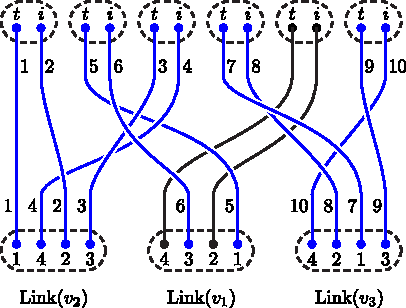
\includegraphics{KoszulFig.pdf} 
\caption{\label{KoszulFig} 
An example of how to compute the Koszul sign $(-1)^{\kappa_\beta}$ diagrammatically  
for a graph consisting of three 0-handles and six 1-handles. 
The lower dashed regions represent the 0-handles, while the upper dashed regions 
represent the 1-handles (with initial and terminal ends marked as $i$ and $t$, respectively). 
The Koszul orderings indicated by the numbers are explained in the text, and 
$\kappa_\beta$ is given by the number of crossings of the blue strands (in this example, 
$(-1)^{\kappa_\beta}=-1$).
\kw{I think we should add crossings between blue strands from different 0-handles, and draw in the even (non-blue) strands}
\kw{Also, I would indicate an ordering of all the strands, not just the odd ones.}
}
\end{figure}


The Koszul sign $(-1)^{\kappa_\beta}$ is defined as follows.
Consider, for fixed $\beta$, the tensor product of the all the super vector spaces
associated to the attaching disks on all the 0-handles.
If there are $k$ 1-handles, then there are $2k$ tensor factors in this tensor product, one 
for each 1-handle end. 
We will compare two different orderings of the tensor factors.
In the first ordering, we place each terminal disk immediately before each initial disk in the ordering.
Such an ordering is well-defined up to even permutations.
In the second ordering, 
we choose a global ordering of the 0-handles and then
use the above choices of local ordering for the factors associated to
each 0-handle
(this is again well-defined up to even permutations, since each 0-handle graph evaluates to zero when the total
parity at that 0-handle is odd).
We then define $(-1)^{\kappa_\beta}$ to be Koszul sign relating these two orderings. 

\medskip

\kw{Note to self: review below again after edits}

We now describe a convenient way to compute $(-1)^{\kappa_\beta}$ graphically, with an 
example shown in Figure \ref{KoszulFig} for a graph consisting of six 1-handles (upper dashed regions) and 3 0-handles $v_1,v_2,v_3$ (lower dashed regions). 
Each 0-handle has four 1-handle attaching regions, which are indicated by the lower small dots and 
which possess an ordering relative to one another (indicated by the numbers within the lower dashed regions). Each attaching 
region can either be even (black) or odd (blue). If it is odd, 
\kw{I would assign, regardless of oddness}
we assign a Koszul ordering to the attaching
region, indicated by the numbers appearing just outside the lower dashed regions.

Each 1-handle either has two even ends or two odd ends: if it has two odd ends, we assign an ordering 
to the ends by placing the terminal end immediately before the initial end in the ordering. This ordering
is denoted by the top row of numbers below the 1-handles in Figure \ref{KoszulFig}. 

To evaluate $(-1)^{\kappa_\beta}$, we draw a fermion line connecting each odd 0-handle attaching region
with Koszul order $k$ to the respective 1-handle end with Koszul order $k$. $(-1)^{\kappa_\beta}$ is then 
simply $(-1)^{n_c}$, where $n_c$ is the number of crossing between fermion lines in the resulting diagram. 
In the example of Figure \ref{KoszulFig} we have $n_c=7$, and so $(-1)^{\kappa_\beta}=-1$. 

\medskip

\kw{we should probably say something about the case with boundary.
at least discuss the Koszul ordering issues.}
\dave{I agree, can attack this once re-visiting the bosonic case.}
\ethan{discussion about boundaries and wavefunctions already kinda exists at the end of the fermionic tensor network part}






\begin{comment}	%% Dave's older version  %%%%%%%%%%%%%%
\dave{Admittedly, this does standardize the 1-handles.
I think it's less confusing when we write down the tensor network to explicitly have the parity matrices on the edges.}
The 1-handle weights are determined by the bilinear pairings given by each 1-handle $e$. 
This pairing is defined by rigidly translating the intitial disk through the 1-handle and and gluing it to the terminal disk across a 2-sphere (with the initial disk having a lower Koszul ordering than the terminal disk).
%This pairing is found from gluing the initial disk to the terminal disk on a sphere and evaluating the net after a translation through the 1-handle. 
While gluing across the 2-sphere it is possible that the spin structures of the two disks differ by a spin automorphism (whose action is encoded in the spin flip functor $(-1)^F$).
\dave{We could also take a path that parallels the edge term in the Hamiltonian section.
} 
%The net to be evaluated is defined with a lower koszul ordering on the initial disk than the terminal disk. 
This spin automorphism is defined by the 1-handle $e$ and the spin structure $\sigma$.
We explicitly write the action of the spin automorphism as $(-1)^{F(e, \sigma)}$ so that the 1-handle weights take the form $(-1)^{F(e,\sigma, \beta)}/\widetilde{\Theta}(e, \beta)$. 
Where $\beta$ is the the labeling of the initial disk, and $F(e, \sigma, \beta)$ is $0$ if $\beta$ has even fermion parity, and $1$ if $\beta$ is odd, 
and the spin structure on the initial and terminal disk differ by a spin flip functor.

%As in the bosonic case, $\widetilde\Theta(e, \beta)$ is defined by the value of the bilinear pairing evaluated on $\mu^*$ and $\mu$, where $\mu^*$ $(\mu)$ 
%is a basis vector in the Hilbert space of the initial (final) attaching end of the 1-handle 
%$e$. In the fermionic case, each vector comes with a Koszul ordering, and 
%we define $\widetilde\Theta$ to only act on edges such that the Koszul ordering
%of the vector $\mu^*$ labeling the initial end of $e$ is exactly one less than that of the vector $\mu$
%labeling the terminal end of $e$. 
%For example, if $e$ has four adjacent 2-handles labeled by $a,b,c,d$ with the orientations of Figure \ref{OneHandlePrime} so that $\mu \in V^{ab^*c^*d}$, then we have \ethan{Dave, would you mind adding a koszul ordering of $k$ to $\mu^*$ (the initial disk vector) and an ordering of $k+1$ to $\mu$ (the terminal disk vector)?}
%\be \widetilde \Theta (e, \beta) =  \Bananafourmu,
%\ee
%where the Koszul ordering is indicated explicitly by the numbers located next to the vertices. 

Additionally, for each 0-handle $v$, $\text{Link}(v,\beta)$ is defined in the same way as in the bosonic case (namely, as the evaluation of a net determined by the 1-handles incident on $v$), 
although now for the evaluation of $\text{Link}(v,\beta)$ to be defined we need to assign an ordering to the vertices of the graph $\text{Link}(v)$.
The 0-handle weights are the evaluation of $\text{Link}(v, \beta)$ with the sign ordering determined by the ordering of the vertices of $\text{Link}(v)$.

Lastly, 
we need to define the Koszul sign $(-1)^{\kappa_\beta}$, whose sole job is to compensate for the arbitrary sign ordering we've given each of the vertices on the 0-handle graphs $\text{Link}(v)$. 
To do so, we first give a global ordering to the 0- and 1-handles.
This then determines a global ordering of the fermions on the 0-handles (since each 0-handle is ordered), 
and independently a global ordering of the fermions on the 1-handles (since each 1-handle is sign ordered from initial to terminal).
We then have,
\begin{align}
(-1)^{\kappa_\beta} = \text{sign} (\sigma)
\end{align}
Where $\sigma$ is the permutation needed to have the two global orderings match (equivalently, $\text{sign}(\sigma)$ is the number of transpositions needed for the two sign orderings to match modulo two). 
Additionally, two global orderings of the 0-handles (1-handles) are related by an even number of transpositions in the sign ordering, 
and so the sign $(-1)^{\kappa_\beta}$ is independent of both global orderings.
Furthurmore, the partition function is independent of the arbitrary ordering assigned the vertices of the 0-handle graphs $\text{Link}(v)$.
To see this, we note that if we change the ordering of the vertices of $\text{Link}(v)$ by a single transposition, then the weight itself will pick up a negative sign (if both labels are odd), 
and the we will have to do one extra transposition to determine the Koszul sign $(-1)^{\kappa_\beta}$. 
Hence the two signs cancel.
(if both or one of the labels are even then the transposition of the ordering in that given 0-handle has no effect on the Koszul sign or the 0-handle weight).
\end{comment}	%% end Dave's older version  %%%%%%%%%



\begin{comment} %%%%%%%%%%%%%%%%
\dave{Plan is to move the following to scrap notes.}
\dave{I am skeptical of the following, 
but wanted to write down the idea while I was thinking about it.
}
We also note that $(-1)^{\kappa_\beta}$ can be written as the evaluation of a diagram in $\text{sVec}$.\footnote{The braided fusion category $\text{sVec}$ has two simple objects which we denote $\unit$ and $\psi$. 
$\psi$ has $\zt$ fusion rules, trivial F-symbols and is a fermion.}
This has the advantage of implicitly modding out by even permutations, and does not require a global ordering of the 0- and 1-handles. 
For each 1-handle that has an odd parity initial disk we draw a graph on the plane with two vertices and one edge labeled by $\psi$.
Next we draw the graphs $\text{Link}(v)$ on the plane. 
We now connect pairs of vertices on $\text{Link}(v)$ with $\psi$ lines if they have odd parity (it is important that no braids are introduced). 
We now ``connect'' the two planar graphs with $\psi$ lines, and evaluate the diagram, see Figure \ref{sVecFig} for an example.
(Note that we are actually taking an inner product between the planar graph defined by the 1-handles, and the planar graph defined by the 0-handles)
\end{comment} %%%%%%%%%%%%%%%%


%%old svec fig
\begin{comment}
\begin{figure}
\begin{centering}
\begin{align}
\nonumber
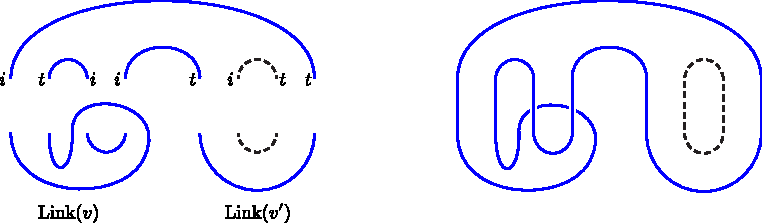
\includegraphics{sVecFig.pdf}
\end{align}
\end{centering} 
\caption{\label{sVecFig}
An example of a Koszul sign $(-1)^{\kappa_\beta}$ written as the evaluation of a diagram in $\text{sVec}$ for a pair of two vertices $v,v'$. 
The upper half of the left figure denotes the 1-handles, with $i$ ($t$) marking the initial (terminal)
edge of the 1-handle.  
The lower half of the left figure shows the two 0-handles, which each have four attached 1-handles.
Solid lines are labeled by $\psi$ and connect two fermion dots with adjacent sign ordering, while dashed lines denote the trivial object. 
The right figure shows the diagram in sVec obtained after connecting the strings on the 0-handles to 
the respective strings on the 1-handles; the evaluation of this diagram determines $(-1)^{\kappa_\beta}$. \ethan{changed the caption a bit to hopefully be a bit clearer}
}
\end{figure}
The evaluation of the diagram can be written as a TVBW state sum, but since we have written the evaluation on the plane, it doesn't sit naturally with the TVBW state sum \eqref{fermionic_tv_sum}.
\dave{Intuition, but haven't checked (Maybe this is Kapustins shadow thing; see \cite{bhardwaj2016}?): 
The combination $(-1)^{\kappa_\beta}(-1)^{F(e, \sigma,\beta)}$ can be written as a TVBW state sum on $M$ with $\mcc = \text{sVec}$.
}
\dave{Could think about:
If $\spc$ is dervied through a fermionic quotient then the parition function can be written as$\cdots$. 
If the Manifold has Boundary then $\cdots$}
\end{comment}


%%%%%%%%%%%%%%%%%%
\subsubsection{The fermionic state sum as a tensor network}
%%%%%%%%%%%%%%%%%%

We now turn to the task of reinterpreting \eqref{fermionic_tv_sum} as a tensor network. %\ethan{replaced ``regularization'' with ``standardization'' since regularization has a different physics meaning}
%\dave{Definitely a good idea.}

\medskip

We incorporate the factors of $d(f, \beta)/n(f,\beta)$ and $\mcd^{-2}$ into the 0-cell 
weights 
in the same way as in the bosonic case. 
As in the bosonic case we denote the dressed 0-handle weights by $\widetilde{\rm Link}(v,\beta)$.
Denoting the modified 0-handle weights by $\widetilde{\rm Link}(v,\beta)$, 
we define the vertex tensor in a similar fashion to \eqref{vertex_tensor}. 
Let $e_1, \cdots, e_k$ be the 1-handles adjacent to the 0-handle $v$ with the same ordering as the vertices of the graph $\text{Link}(v)$.
Let $V_i$ be defined in the same way as \eqref{0_handleVectorspaces} (with the modification that $V_i$ is a super vector space).
We define 
\begin{align} 
T_v  \in V_1^* \tp \cdots \tp V_k^*
\end{align}
by 
\begin{align}
T_v(w_1 \tp \cdots w_k) = \widetilde{\text{Link}}(v, w_1 \tp \cdots \tp w_k)
\end{align} 
where $w_i \in V_i$.
In words, $T_v$ evaluates the string-net graph determined by $\text{Link}(v)$ with the ordered vertices labeled by $w_1, \cdots, w_k$ (in the same order), and multiplied by the appropriate factors of $d(f,\beta)$ and $\mcd^{-2}$.

The partition function 
is the same as in the bosonic case, being computed as a trace of the $T_v$ tensors:
\be \label{fermion_Z_as_tr} Z(M) = \tr \left(\bigotimes_{v\in \mch_0} T_v\right).\ee
where the trace is denotes denotes the sum over all contracted 1-cell labelings normalized by $\widetilde{\Theta}^{-1}$.
%The tensor trace is defined so that we insert a parity matrix $(-1)^{F(e, \sigma)}$ on every 1-cell, and a $\widetilde{\Theta}$ symbol normalization in the contraction. 
In practice, to perform the trace, we require that the sign ordering on the pair of vectors to be contracted over have adjacent sign orders (with terminal lower than initial). 
%In practice, to perform the contraction, the we require the pair of vectors being contracted over to have adjacent Koszul ordering (i.e., initial to terminal).
To get the pair of vectors in adjacent sign ordering we need to apply a number of Koszul isomorphisms. 
After contracting all vectors we pick up the appropriate factor of $(-1)^{\kappa_\beta}$. 
Again, $Z(M)$
is independent of the way we assign factors of $d(f,\beta)$ and $\mcd^{-2}$ to the 
vertex tensors. 
If $\bd M$ is non-empty, we again follow the bosonic prescription in \eqref{trace_pM_nonempty} 
to obtain $Z(M) = \tr \left( \bigotimes_{v\in \mch_0} T_v \right) \in W_1^*\tp\cdots\tp W_n^*$, where 
$W_1, \ldots, W_n$ are the vector spaces associated to the boundary 0-cells and we 
are implicitly making use of the undordered tensor product. When using $Z(M)$ to compute 
amplitudes of different string-net boundary conditions, care must be taken when performing the 
tensor contraction on ordered representatives because of Koszul sign issues. 

\ethan{un-commented the following since I still think we should include a contraction example, either here 
or possibly in defn section}

We will now elaborate on how to perform tensor contractions in the fermionic setting. 
When we contract out two tensor indices of a tensor in $\mch^*\tp\mch$, we must be careful to only perform 
the contraction on two tensor factors that have adjacent Koszul ordering in the tensor product.
For example, suppose we have two tensors $Q \in V_Q$ and $T\in V_T$,
defined by
\begin{align}
Q &= \sum_{q_L \tp q \tp q_r } Q(q_L \tp q \tp q_R)q_L \tp q \tp q_R,\\
T &= \sum_{t_L \tp t \tp t_R} T(t_L \tp t \tp t_R  )t_L \tp t \tp t_R,
\end{align}
where we have split the vector spaces $V_Q$ and $V_T$ into tensor factors on 
the left and right of the two indices that we would like to contract, namely $t \in V$ and $q \in V^*$.
We define the contracted tensor by $K$, which is given by
\begin{align}
K = \sum_{ q_L \tp q_R \tp t_L \tp t_R}K(q_L \tp q_R \tp t_L \tp t_R) q_L \tp q_R \tp t_L \tp t_R,
\end{align} 
with 
\begin{align}
\label{contraction_example}
K(q_L \tp q_R \tp t_L \tp t_R) &= \sum_{q,t} Q(q_L \tp q \tp q_R)R(t_L \tp t \tp t_R  ) (-1)^{|q| |q_r|}(-1)^{|t_L| | t|} \delta_{q^*,t}\\
&= \sum_{t} Q(q_L \tp t^* \tp q_R)R(t_L \tp t \tp t_R  ) (-1)^{|t|( |q_R| +|t_L|)}.
\end{align}
In the above, we have used the fact that $\delta_{q^*,t}$ is only non-zero
if $|q|=|t|$. 
The Koszul sign $(-1)^{|t|( |q_R| +|t_L|)}$ is picked up from commuting the tensor factors $q$ and $t$ next to one another, so that they have the correct Koszul ordering for being input into the contraction map. 

\ethan{I found the following very useful for avoiding confusion, but it's likely not strictly needed}
In the above examples, we have used the implicit left-to-right Koszul ordering convention.
In practice, we will more often be performing a contraction on a series of tensors whose Koszul
orderings are indicated explicitly by numerical subscripts, since this notation is better suited to 
our diagrammatic formalism. For example, we have 
\be Q\tp T = \sum_{q_L \tp q \tp q_r } Q(q_L \tp q \tp q_R)T(t_L \tp t \tp t_R  ) q_{L1} \tp q_2 \tp q_{R3} \tp t_{L4} \tp t_5 \tp t_{R6}.\ee
We would like to contract out the indices $t\in V,q\in V^*$, but in order to do this they must have adjacent Koszul ordering. 
To obtain such an 
order, we use the following manipulations:
\begin{align} q_2 \tp q_{R3} \tp t_{L4} \tp t_5 & = (-1)^{|q||q_R|}q_3 \tp q_{R2} \tp t_{L4} \tp t_5 \\ & = (-1)^{|q||q_R|+|t||t_L|} q_3 \tp q_{R2} \tp t_{L5} \tp t_4.
\end{align}
We are now ready to contract out the $q$ and $t$ indicies. The Koszul sign we pick up, namely 
$(-1)^{|q||q_R|+|t||t_L|}$, is of course the same as the one obtained with the implicit left-to-right Koszul ordering convention. 

In summary, the Koszul sign that appears when performing the tensor contraction in the evaluation of $Z(M)$ can be found 
by ensuring that tensor factors 
being contracted always have adjacent Koszul-ordering and by using \eqref{contraction_example} repeatedly.



%%%%%%%%%%%%%%%%%%%%
\subsubsection{Fermionic standardization procedures}
%%%%%%%%%%%%%%%%%%%%

As in the bosonic case, we may employ a standardization 
procedure in which all vertices in the string nets assigned to the 0-handles are in the pitchfork form.
This standardization procedure results in nets on 0-handles which are all standardized independently of one another: 
the form of a given trivalent vertex at the initial edge of a 1-handle $e$
and the form of the associated vertex on the terminal edge of the 1-handle may be related by a pivot operation.
Properly accounting for this requires inserting pivot operators $P_e=P^{l_e}$ into the 
1-handles, as in \eqref{horshoe_resln}. 
Rather than tacking the spin-structure signs onto the 0-handle weights 
(as we did in the state sum described above) we incorporate them into the pivots.
Indeed, we now have $P_e^3=(-1)^F$, so that $l_e$ is 
valued in $\zz_6$ as opposed to $\zz_3$ (alternatively, we could keep $l_e \in \zz_3$  but insert $(-1)^{F} \cdot P^{l_e}$ where appropriate).
We keep the spin framing at the 0-handles fixed by virtue of the pitchforkization procedure (and require that every 0-handle is related by a translation), 
the spin structure of the underlying 3-manifold is encoded in the edge pivots $P_e$ (and the standardized 0-handles).
\dave{The following may need to be done more carefully}
The attachment regions of the 0-handles are also related by spin diffeomorphisms, 
in this case either $\text{id}$ or $(-1)^F$. 
If we multiply all the pivots along a closed path (including those coming from the 0-handles) then they must equal $(-1)^F$ if the 
path is bounding and $+1$ if the path is non-bounding.

Lastly, we note that if we further require the cell decomposition to be dual to a triangulation, 
then we can choose the 0-cell weights to that a take a similar form to\eqref{Bosonic_tet}.
The modification is that the vertices of $\text{Link}(v)$ must be ordered, 
so that 
\begin{align} 
	%T_v = \TetrahedronPrime \; \cdot \alpha \tp \beta \tp \gamma \tp \delta, 
	T_v(\alpha \tp \beta \tp \gamma \tp \delta) = {\rm Tet}(v,\alpha \tp \beta \tp \gamma \tp \delta) = \Tetrahedron.
\end{align}
Note that there are still multiple versions of the standardized tetrahedral weights ${\rm Tet}$ differing by choices of the edge orientations.
The fermionic analogue of \eqref{bos_tv_sum_std} can now be written:
\begin{align}
\label{ferm_tv_sum_std}
	Z(M) = \sum_{\beta\in\mcl(\mch)}(-1)^{\kappa_\beta}
		\prod_{c\in\mch_3} \mcd^{-2}
		\prod_{f\in\mch_2} \frac{d(f, \beta)}{n(f,\beta)}
		%\prod_{e\in\mch_1} \frac{ (-1)^{F(e,\sigma, \beta)}}{ \widetilde \Theta(e, \beta)}
		\prod_{e\in\mch_1}  \widetilde \Theta(P_e, \beta)^{-1}
		\prod_{v\in\mch_0} \text{Tet}(v, \beta) .
\end{align}
Again, $\widetilde{\Theta}(P_e, \beta)$ is a standard pairing as in \eqref{reflection_pairing_defn} but modified by the pivot isomorphism $P_e = P^{l_e}$.




%%%%%%%%%%%%%%%%%%%%%%%%%%%%%%%%%%%
\subsection{The shadow world and ground state wave functions}
%%%%%%%%%%%%%%%%%%%%%%%%%%%%%%%%%%%
\dave{I haven't been through this section in recently (Aug 11)}
\dave{Have been through part of this section.}
\ethan{some notational things still need to be updated to reflect new state-sum notation}

\ethan{still might need to mention connection to MPO's/mention tube category/excitations}



In this subsection we define a tensor network that produces the ground state wave function of the Hamiltonian defined in \eqref{ham}.
To do so, we evaluate $Z(M)$ on manifolds of the form $M =\Sigma \times [0,1]$ using the 
state-sum technology developed in the previous sections\footnote{Historically, this version of the state sum 
pre-dates TVBW and was first found by Kirillov and Reshetikhin~\cite{Kirillow1989} who coined the term 
`shadow world', which was later extended by Turaev~\cite{turaev1992shadow} and included shadows of links 
which he coined `shlinks'. \ethan{the gratuitous reference to shlinks is fun but not strictly needed}.}. 
We will take $\Sigma$ to be a two-dimensional spin surface in what follows, although 
the approach we describe can easily be modified to work for one-dimensional spin manifolds as well. 

The basic input to the wave-function is the same as that of the Hamiltonian defined in \eqref{ham}, namely 
a super pivotal category $\spc$, an oriented spin surface $\Sigma$, and a cell decomposition of $\Sigma$.
We fix the cell decomposition at $\Sigma \times \{ 1 \} $ (which we denote by $\Sigma_1$) to match the cell decomposition which we use in the Hamiltonian \eqref{ham}.
%We will be evaluating partition functions on the manifold $\Sigma \times [0,1]$, where the cell decomposition on the slice $\Sigma \times \{ 1 \} $ (which we denote by $\Sigma_1$)
%is fixed to be the cell decomposition on which we wish to define the Hamiltonian \eqref{ham}. 

We also fix a cell decomposition of $\Sigma \times \{0\}$, which we denote $\Sigma_0$.
Different choices of boundary conditions on $\Sigma_0$ lead to wavefunctions built
over different ground states in the theory. 
\dave{Wavefunctions built over different ground states sounds funny. 
}

The partition function provides a linear map between the Hilbert spaces at $\Sigma_0$ and $\Sigma_1$:
\begin{align}
Z(\Sigma_{0\ra1} ): \; \mch(\Sigma_0) \ra \mch(\Sigma_1).
\end{align}
\dave{Did we get rid of $\mch(\Sigma)$ notation?}
The image of this map is the space of ground states of \eqref{ham}.
Explicitly, we can prepare wave functions out of a fixed input state $v_0\in \mch(\Sigma_0)$ by
%\begin{align}
%
%\ket{\Psi} = \sum_{ v_1 \in \mch(\Sigma_1)} \ket{v_1} v_1^* \cdot Z(\Sigma_{0\ra1} ) %\cdot v_0.
%\end{align} 
\begin{align}\label{GroundState}
\ket{\Psi} = \sum_{v_1 \in \mch(\Sigma_1)} \ket{v_1} Z(\Sigma_{0\ra1}; v_0, v_1),
\end{align}
where $Z(\Sigma_{0\ra1}; v_0, v_1)$ is the evaluation of the partition function with 
boundary conditions fixed by $v_0$ and $v_1$. 
If the states $v_0$ and $v_1$ are in different ground state sectors, then $Z(\Sigma_{0\ra1};v_0,v_1)=0$. 
%Depending on the topology of $\Sigma$ and the input super tensor category, the ground state of the theory 
%will generically be degenerate, with the choice of $v_0$ and $\Sigma_0$ determining which ground state
%the wave function is built upon. 

\begin{figure}
\begin{center}
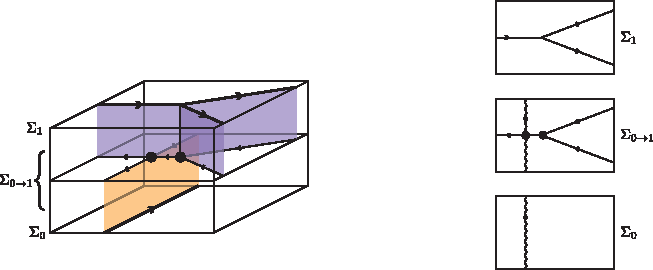
\includegraphics{CellDecomposition.pdf}
\caption{\label{CellDecomposition}
\dave{Will pitchforkize.} \ethan{Actually, I think it might be clearer if you don't. We mention the standardization procedure after we talk about the cell decomposition extension, and I think the figure is easier to look at pre-pitchforkization} 
The decomposition used to construct the shadow world tensor network, shown 
in its pre-standardized, pre-pitchforkization state.
The top layer $\Sigma_1$ is the cell decomposition that we use to construct the Hamiltonian in \eqref{ham}.
The bulk cell decomposition $\Sigma_{0\ra1}$ is found by extending $\Sigma_0$ into 
$\Sigma \times [0,\frac{1}{2}]$, and $\Sigma_{1}$ into $\Sigma \times [\frac{1}{2},1]$ (left figure).
The input cell decomposition $\Sigma_0$ is taken to be in `normal' position with respect to $\Sigma_1$, meaning that when each cell decomposition is extended into the bulk, the two decompositions only intersect transversely along edges. 
On the right, we have shown two dimensional representations of small patches of the cell decomposition. 
In the two dimensional pictures we will denote the cells stemming from $\Sigma_0$ by squiggly lines.
Notice that the orientation of all lines on $\Sigma_{0 \ra1}$ have been reversed relative to $\Sigma_0$ and $\Sigma_1$. 
}
\end{center}
\end{figure}

In order to evaluate $Z(\Sigma_{0\ra1}; v_0, v_1)$, we need to specify a cell decomposition on $\Sigma_{0\ra 1}$ (although the actual partition function is independent of the particular choice). 
We can take the cell decomposition in the bulk of $\Sigma_{0\ra1}$ to be any cell decomposition that agrees with the cell decomposition of $\Sigma_0$ and $\Sigma_1$ when restricted to $\partial \Sigma_{0\ra1}$.
However, there is a particularly convenient choice, which corresponds to extending the cell decomposition of $\Sigma_0$ into $\Sigma \times [0, 1/2]$, and that of $\Sigma_1$ into $\Sigma \times [1/2, 1]$, see Figure~\ref{CellDecomposition}. 
When we do this extension, every $k$-cell in $\Sigma_0$ and $\Sigma_1$ is extended into a $(k+1)$-cell in the bulk 
of $\Sigma_{0\ra1}$ (the $(k+1)$-cells are the `shadows' of the $k$-cells, and hence the bulk constitutes the `shadow world'\dave{never made that connection before, is that why they called it the shadow world?}). 
It is convenient to take the two cell decompositions on $\Sigma_0$ and $\Sigma_1$ to be in `normal' position,
meaning that the extension of $\Sigma_0$ into the bulk only intersects the extension of $\Sigma_1$ transversely along edges, again see Figure~\ref{CellDecomposition}.


We now specify the amplitude $Z(\Sigma_{0\ra 1}; v_0, v_1) $ in \eqref{GroundState}.
The amplitude is determined using the state sum procedure developed previously, and as such we will be brief in what follows. 
The labels of the 2-cells that extend from $\Sigma_0$ and $\Sigma_1$ are determined by $v_0$ and 
$v_1$, since they are the shadows of 1-cells in $\Sigma_0$ and $\Sigma_1$. 
The 2-cell labels living at $\Sigma \times \{ 1/2 \}$ are not fixed as input data however, and need to be 
summed over.
\dave{Should probably conform with notation in previous section}

As was done in our treatment of the state sum, to construct the weights ${\rm Link}(v,\beta)$ for a given 0-cell $v$ in $\Sigma \times \{1/2\}$, we insert a small $S^2$ around 
$v$ and examine the intersections of neighboring 2-cells with the $S^2$. These intersections 
are marked on the $S^2$ as edges, and the ${\rm Link}(v,\beta)$ are formed by evaluating 
the picture formed by these edges. 
\dave{Do we need to describe what $\text{Link}(v,\beta)$ is?}

\begin{figure}
\begin{center}
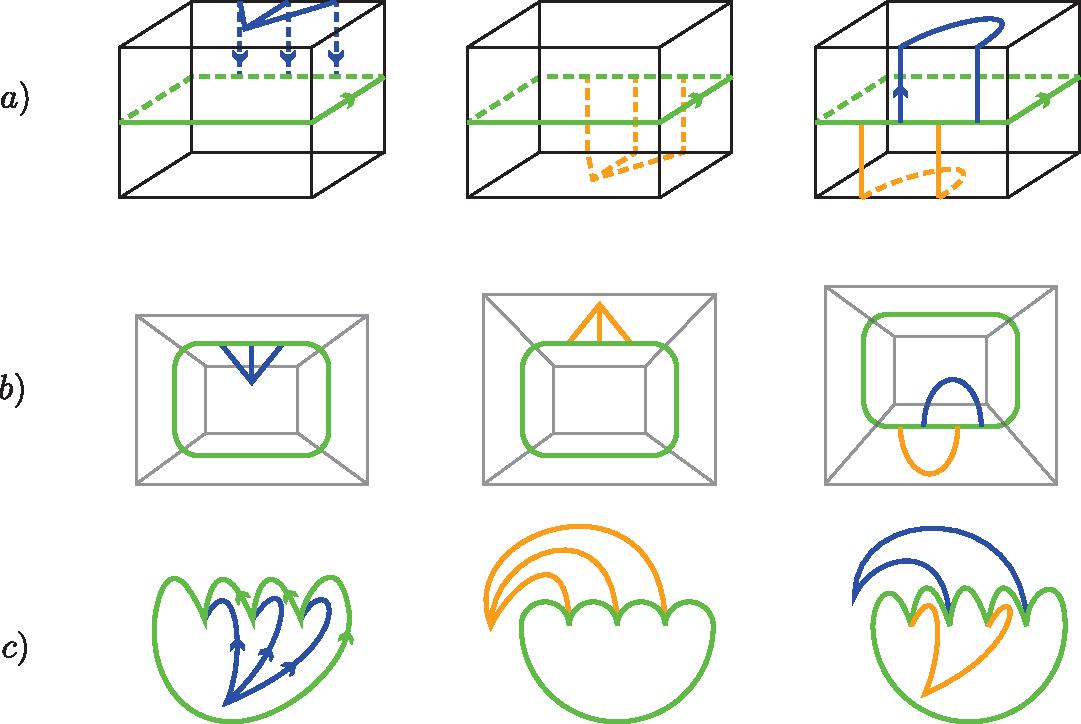
\includegraphics[scale=0.6]{StandardizedSlabTensors.pdf}
\caption{\label{StandardizedSlabTensors}
In row a) we show the three kinds of possible 0-cell tensors that could appear in the tensor contraction when 
computing the partition function $Z(\Sigma;v_0,v_1)$. The cube is drawn so that the 0-cell is located in the cube center. 
Blue (orange) lines represent intersections of 2-cells in the extension of the cell decomposition $\Sigma_1$ ($\Sigma_0$) with the cube, and 
green lines represent intersections of 2-cells in $\Sigma \times \{1/2\}$ with the cube. 
In row b) we show the first step for one possible standardization procedure, where the diagrams 
have been drawn projected into two dimensions. 
In row c) we finish the standardization of the diagrams by making each trivalent vertex a pitchfork. The appropriate 0-cell 
tensors are found by evaluation of these diagrams. 
}
\end{center}
\end{figure}

By looking at Figure~\ref{CellDecomposition}, we see that there are only three kinds of 0-cells that show up in 
$\Sigma \times \{1/2\}$: those that are formed at the x-shaped intersection of a 1-cell in the extension of $
\Sigma_0$ with a 1-cell in the extension of $\Sigma_1$, those where a 0-cell in the extension of $\Sigma_0$ 
meets the interior of a 2-cell in 
the extension of $\Sigma_1$, and vice versa. These possibilities lead to three different types of 0-cell weights that need to be evaluated. 
These three possibilities are illustrated in the top row $a)$ of Figure \ref{StandardizedSlabTensors}, where we have drawn a cube surrounding the 0-cell instead of an $S^2$.
In the figure, the blue (orange) lines denote 
the intersections of 2-cells in $\Sigma \times (1/2,1]$ (in $\Sigma \times [0,1/2)$) with the cube, 
and the green lines denote the intersection of 2-cells in $\Sigma \times \{1/2\}$ with the cube. 
The orientation of the lines drawn in these figures is fixed by the orientations of each of the 2-cells, 
which are determined with the aid of the orientation of $\Sigma$. 
In order to facilitate computations, we will need to standardize these diagrams according to the 
usual `pitchforkization' procedure employed in the previous sections. 
To do the standardization, we first project the diagrams into the plane (shown in the second row 
of Figure \ref{StandardizedSlabTensors}), and then deform each of the trivalent vertices 
to pitchforks. The final standardized diagrams are displayed in the third row of Figure \ref{StandardizedSlabTensors}.

The evaluation of these standardized diagrams gives the weight appearing in the partition function. 
Explicitly, for a 0-cell $v$ involving three neighboring 2-cells from the extension of $\Sigma_1$ (left column of row $a)$ in Figure \ref{StandardizedSlabTensors}, we assign the weight ${\rm Link}(v,\beta)$ as follows:
\begin{align}
\Tensora \; \ra {\rm Link}(v,\beta) &= \;  \Tensoraa %\cdot \mu_0 \tp s_1 \tp s_2 \tp s_3.
\end{align}
where $\beta$ denotes the labels provided by the indices $\mu_0,s_1, s_2, s_3$.

In the diagrams, the green letters $A,B,C$ denote the labels of the 2-cells in $\Sigma \times \{1/2\}$, which will 
be summed over when computing the amplitude $Z(\Sigma_{0\ra1}; v_0, v_1)$. The labels of 
the blue lines are fixed however, and determined by the labels of the 2-cells which are shadows of 1-cells 
in $\Sigma_1$. 

Weights for the other types of 0-cells in $\Sigma \times \{1/2\}$ are determined similarly. For the type of 
0-cell in the center column of row $a)$ in Figure \ref{StandardizedSlabTensors}, we assign the weight
\begin{align}
\Tensorc \;\ra {\rm Link}(v,\beta) &= \; \Tensorcc % \cdot \nu_0 \tp s_1 \tp s_2 \tp s_3, \\
\end{align}
while for the type of 0-cell in the last column we assign the weight
\begin{align}
\Tensorb \; \ra {\rm Link}(v,\beta) &= \;  \Tensorbb  %\cdot s_0 \tp s_1 \tp s_2 \tp s_3, \\
\end{align}
which corresponds to a string operator. 
%In all of these weig, we are making use of the implicit left-to-right Koszul ordering convention for the 
%tensor factors. 
\dave{I think we should write these as tensors. 
We should also specify which vertices pick up a $(-1)^{|\mu|}$.} 

In order to perform the contraction that will compute the partition function, all the 1-cells 
$\Sigma \times \{1/2\}$ need an orientation. Since these 1-cells biject with the 1-cells of $\Sigma_0$ and $\Sigma_1$ (they are all shadows of 1-cells in either $\Sigma_0$ or $\Sigma_1$ from our 
choice of cell decomposition in $\Sigma_{0\ra1}$), we can assign an orientation to each 1-handle in 
$\Sigma \times \{1/2\}$ using the orientation of the 1-cells in $\Sigma_0$ and $\Sigma_1$, which 
are fixed by the states $v_0$ and $v_1$.

We can now compute $Z(\Sigma_{0\ra1}; v_0, v_1)$ 
using the state sum: 
\begin{align} 
Z(\Sigma_{0\ra1}; v_0, v_1) = \sum_{ \beta\in\mcl(\mch^{1/2})_{bulk}}  (-1)^{\kappa_\beta} \prod_{f \in \mch^{1/2}_2} \frac{d(f,\beta)}{n(f,\beta)} 
\prod_{e \in \mch^{1/2}_1} \widetilde{\Theta}(P_e,\beta)^{-1} \prod_{v \in \mch^{1/2}_0} {\rm Link}(v,\beta),
\end{align} 
where we have used $\mch^{1/2}_k$ to denote the collection of $k$-cells in $\Sigma \times \{1/2\}$ and $\mcl(\mch^{1/2})_{bulk}$ 
to denote colorings of the bulk degrees of freedom in $\Sigma_{0\ra1}$. 
